%%%%%%%%%%%%%%%%%%%%%%%%%%%%%%%%%%%%%%%%%%%%%%%%%%%%%%%%%%%%%%%%%%%%%%%%%
% ARTICLE ABOUT FATE OF SYNONYMOUS MUTATIONS IN HIV
%%%%%%%%%%%%%%%%%%%%%%%%%%%%%%%%%%%%%%%%%%%%%%%%%%%%%%%%%%%%%%%%%%%%%%%%%
\documentclass[12pt,a4paper,notitlepage,onecolumn]{article}
%%%%%%%%%%%%%%%%%%%%%%%%%%%%%%%%%%%%%%%%%%%%%%%%%%%%%%%%%%%%%%%%%%%%%%%%%
\newcommand{\Author}{Fabio~Zanini and Richard~A.~Neher}
\newcommand{\Title}{(Rise and fall of synonymous mutations)}
\newcommand{\Keywords}{{HIV}, {synonymous}, {population genetics}}
%%%%%%%%%%%%%%%%%%%%%%%%%%%%%%%%%%%%%%%%%%%%%%%%%%%%%%%%%%%%%%%%%%%%%%%%%
\usepackage[english]{babel}
\usepackage[utf8x]{inputenc}
\usepackage{amsmath,amsfonts,amssymb,eucal,eurosym}
\usepackage{color}
\usepackage{subfig}
\usepackage{graphicx}
\usepackage[font=small, format=hang, labelfont={sf,bf}, figurename=Fig.]{caption}
\usepackage{natbib}
\usepackage{pslatex}
\usepackage[colorlinks,linkcolor=red,citecolor=red]{hyperref}
\hypersetup{pdfauthor={\Author}, pdftitle={\Title}, pdfkeywords={\Keywords}}
%%%%%%%%%%%%%%%%%%%%%%%%%%%%%%%%%%%%%%%%%%%%%%%%%%%%%%%%%%%%%%%%%%%%%%%%%
\graphicspath{{./figures/}}
%%%%%%%%%%%%%%%%%%%%%%%%%%%%%%%%%%%%%%%%%%%%%%%%%%%%%%%%%%%%%%%%%%%%%%%%%
%\DeclareMathOperator\de{d\!}
\newcommand{\comment}[1]{\textit{\textcolor{red}{#1}}}
\newcommand{\mut}{u}
\newcommand{\mfit}{\langle F\rangle}
\newcommand{\mexpfit}{\langle e^{F}\rangle}
\newcommand{\ox}{r}
\newcommand{\co}{\rho}
\newcommand{\gt}{g}
\newcommand{\locus}{s}
\newcommand{\locuspm}{t}
\newcommand{\OO}{\mathcal{O}}
%%%%%%%%%%%%%%%%%%%%%%%%%%%%%%%%%%%%%%%%%%%%%%%%%%%%%%%%%%%%%%%%%%%%%%%%%
\title{\Title}
\author{\Author}
\date{\today}
%%%%%%%%%%%%%%%%%%%%%%%%%%%%%%%%%%%%%%%%%%%%%%%%%%%%%%%%%%%%%%%%%%%%%%%%%
\begin{document}
%%%%%%%%%%%%%%%%%%%%%%%%%%%%%%%%%%%%%%%%%%%%%%%%%%%%%%%%%%%%%%%%%%%%%%%%%
\maketitle

\begin{abstract}
\noindent
Intrapatient HIV evolution is goverened by selection on the protein level in the
arms race with the immune system (killer T-cells and antibodies). Synonymous
mutations do not have an immunity-related phenotype and are often assumed to be
neutral. In this paper, we show that synonymous changes in epitope-rich regions
are often deleterious but still reach frequencies of order one.  We analyze time
series of viral sequences from the V1-C5 part of {\it env} within individual
hosts and observe that synonymous derived alleles rarely fix in the
viral population. Simulations suggest that such synonymous mutations
have a (Malthisuan) selection coefficient of the order of $-0.001$, and that
they are brought up to high frequency by linkage to neighbouring beneficial
nonsynonymous alleles (genetic draft). As far as the biological causes are
concerned, we detect a negative correlation between fixation of an allele and
its involvement in evolutionarily conserved RNA stem-loop structures.
This phenonenon is not observed in other parts of the HIV genome, in which
selective sweeps are less dense and the genetic architecture less constrained.
\end{abstract}

\section{Introduction}
\section{Results}

\begin{figure}
\begin{center}
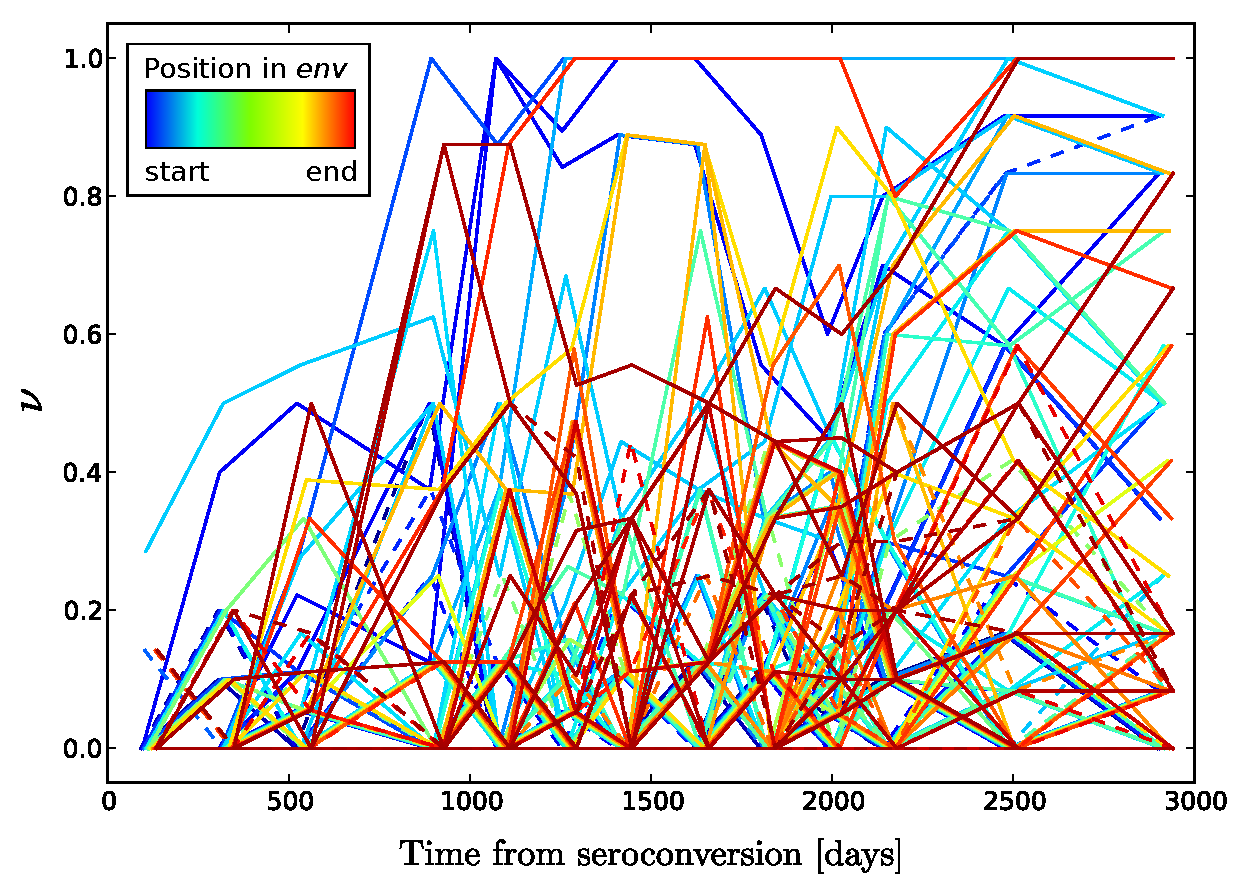
\includegraphics[width=\linewidth]{Shankarappa_allele_freqs_trajectories_syn_nonsynp8}
\caption{Allele frequency trajectories of typical patient, C3-V5, nonsynonymous
(solid) and synonymous mutations (dashed lines). Most synonymous mutations are
not fixed.}
\end{center}
\end{figure}

\begin{figure}
\begin{center}
\subfloat{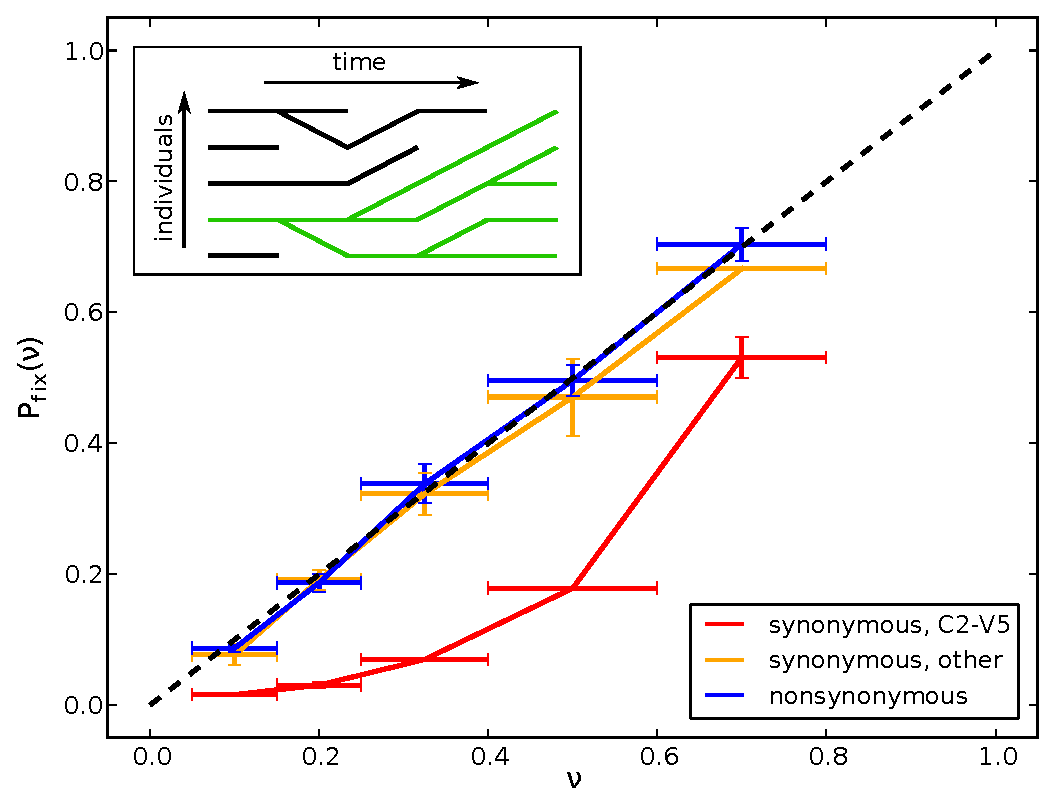
\includegraphics[width=0.49\linewidth]{Bunnik2008_fixmid_syn_ShankanonShanka}}
\subfloat{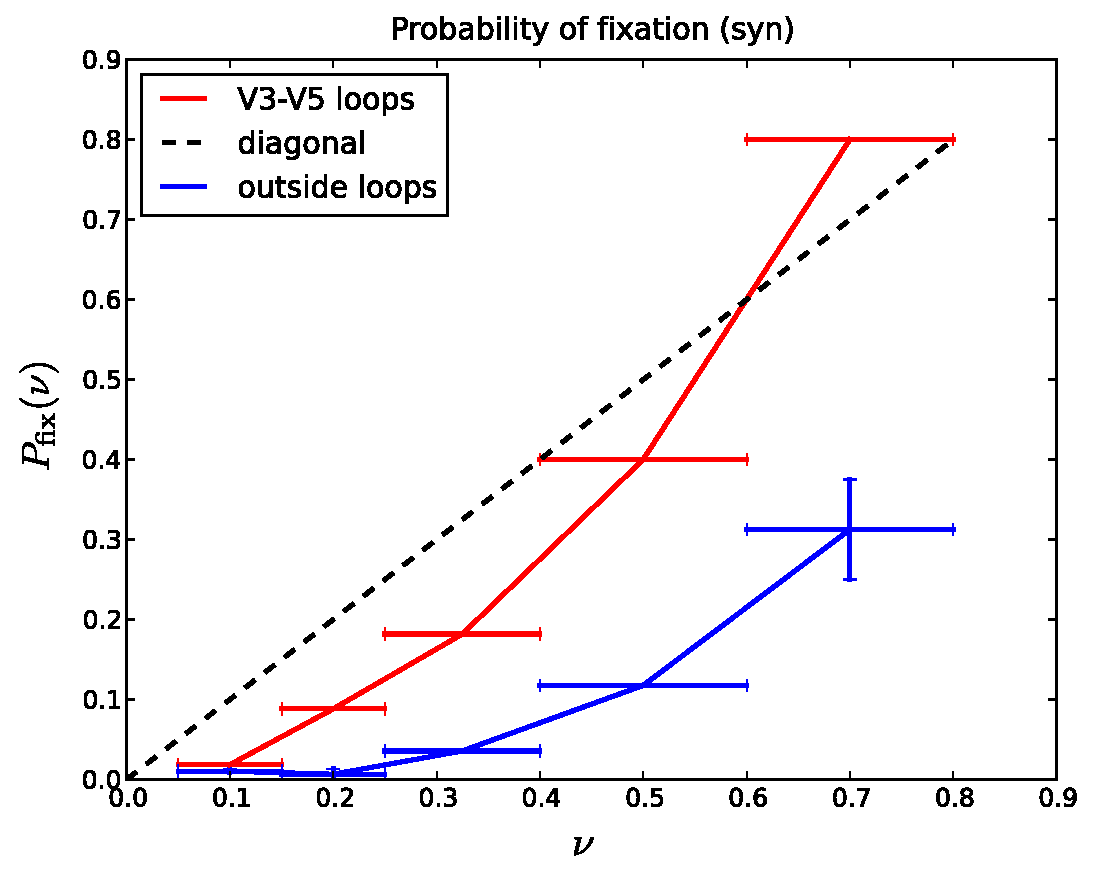
\includegraphics[width=0.49\linewidth]{Shankarappa_fixmid_syn_V_regions}}
\caption{Fixation probability of derived synonymous alleles is strongly
suppressed in C3-V5 versus other parts of the {\it env} gene (left panel).
Especially hard is fixation of new alleles in conserved regions flanking the V
loops (right panel). The black dashed line is the prediction from neutral
theory, for comparison purposes.}
\end{center}
\end{figure}

\begin{figure}
\begin{center}
\subfloat{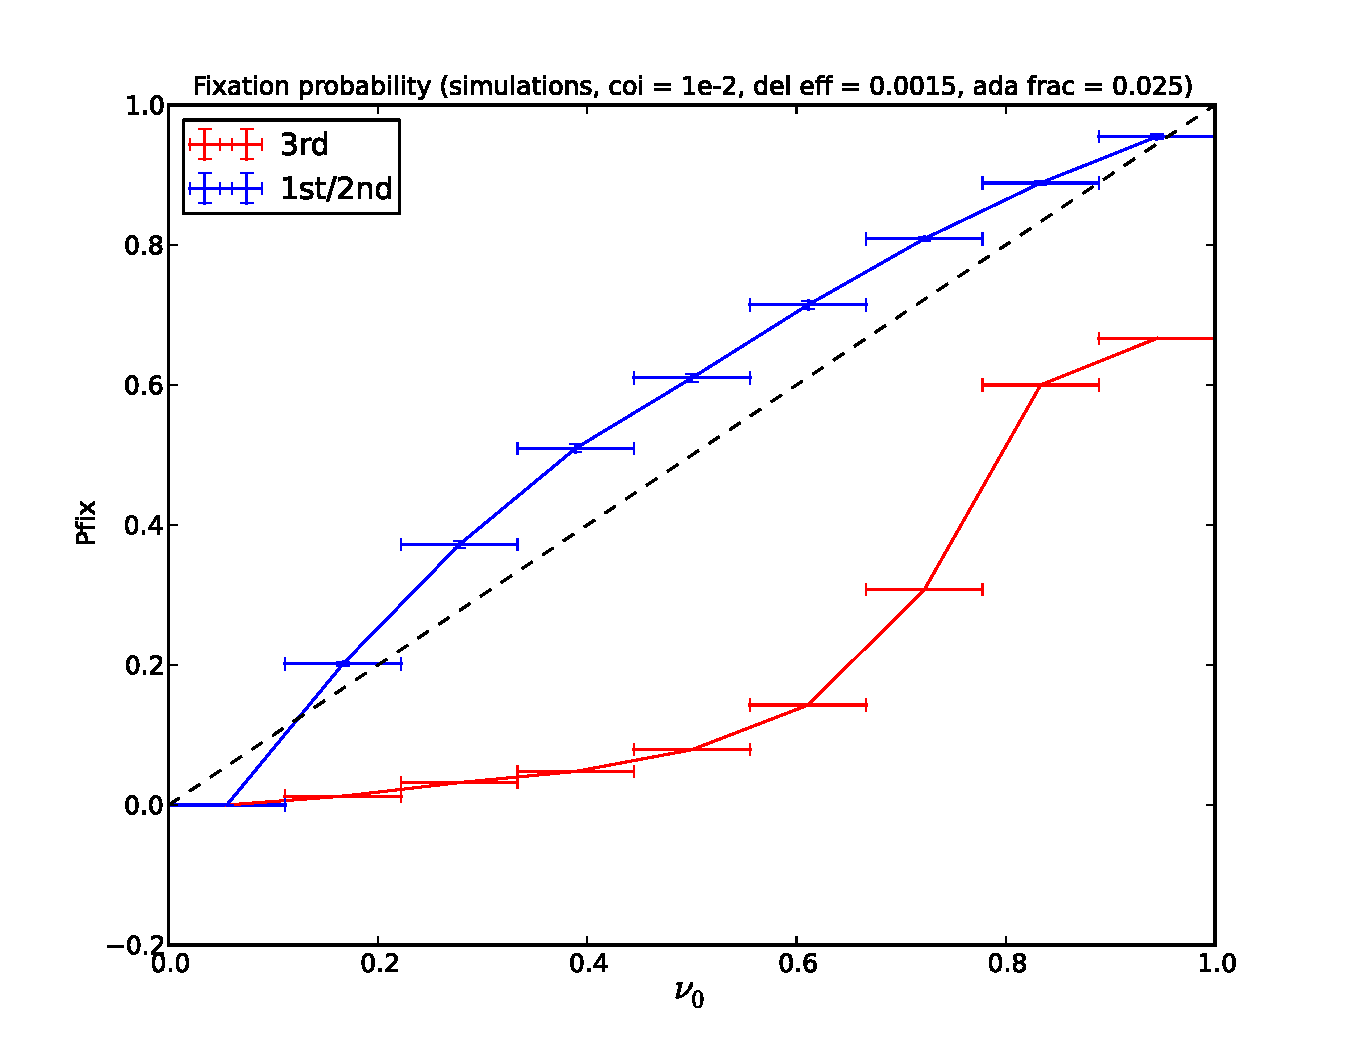
\includegraphics[width=0.49\linewidth]{fixation_probability_shortgenome_N_1e4_epitopes_example_longer}}
\subfloat{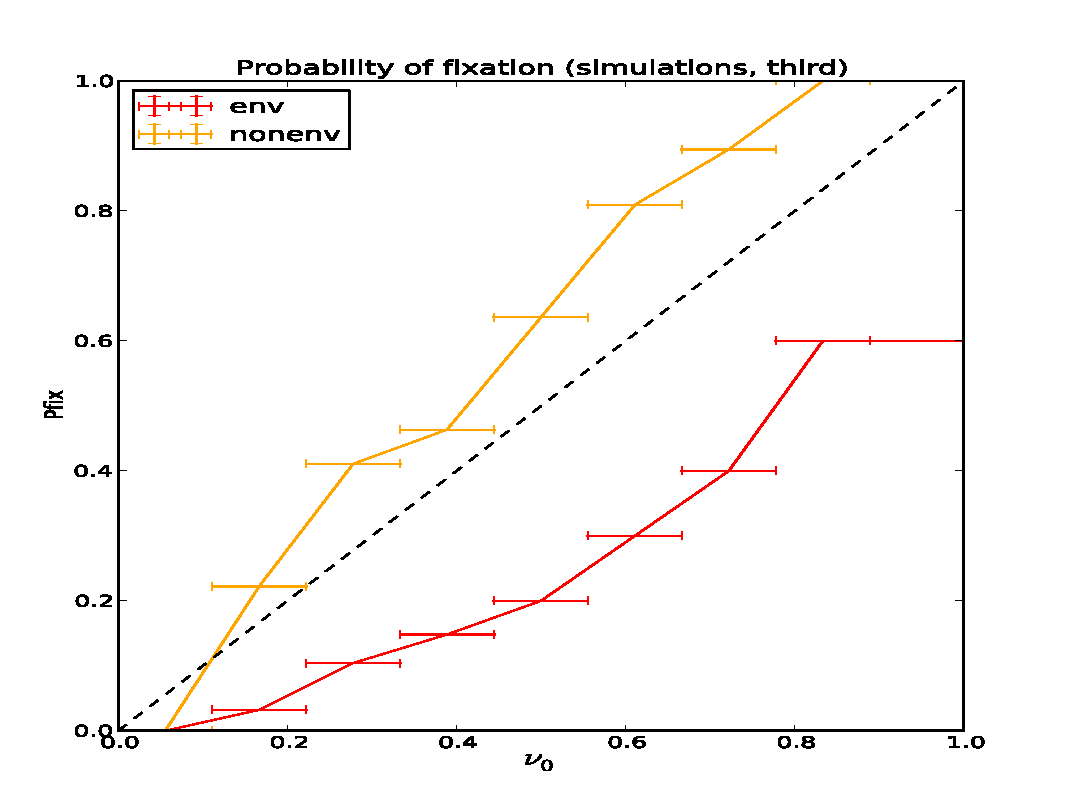
\includegraphics[width=0.49\linewidth]{fixation_probability_N_1e4_3ingredients_3rddel_envnonenv_stopall}}
\caption{Simulations show that the suppression of fixation probability can be
generated by linkage to sweeping nonsynonymous alleles nearby. Two possible
scenarios are competition between escape mutants (left panel) and time-dependent
selection due to immune sytem recognition (right panel).}
\end{center}
\end{figure}

\begin{figure}
\begin{center}
\subfloat{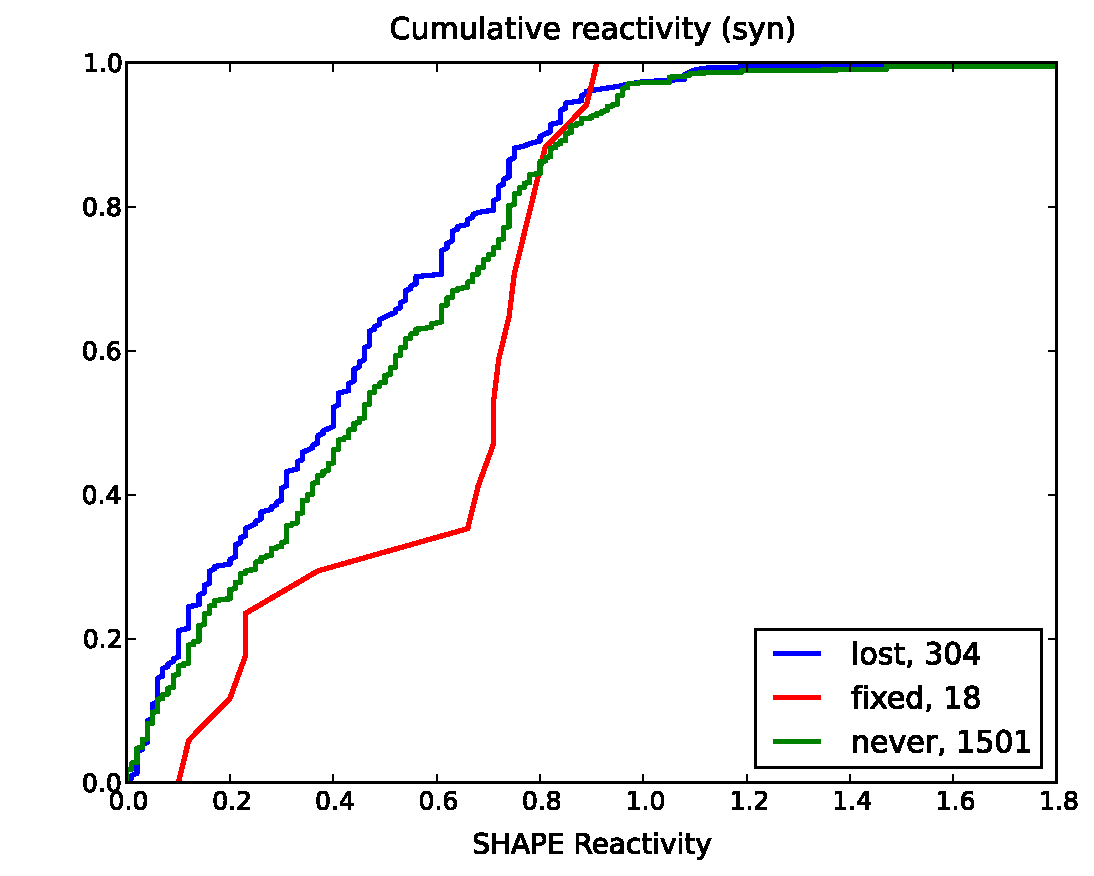
\includegraphics[width=0.49\linewidth]{mixed_Shankarappa_Bunnik2008_Liu_fixation_reactivity_Vandflanking_fromSHAPE}}
\subfloat{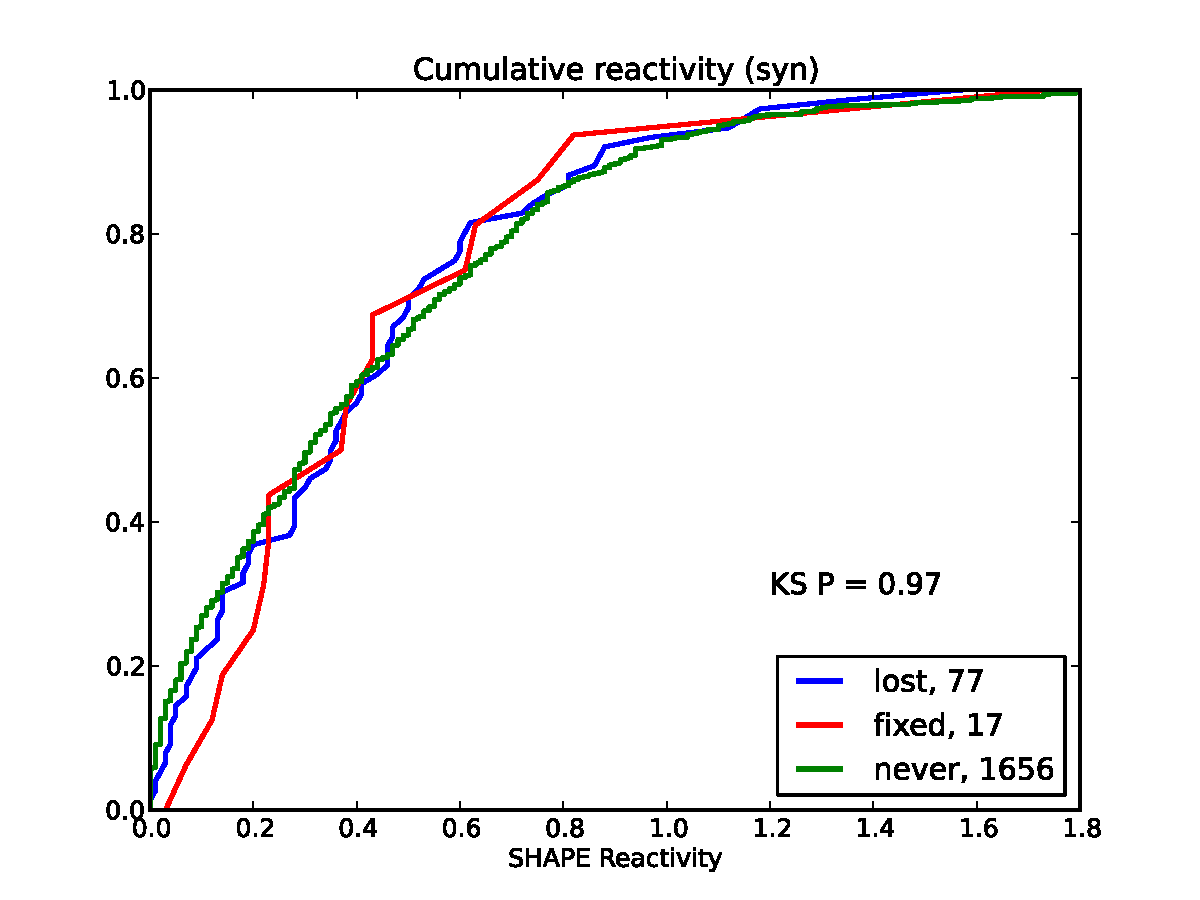
\includegraphics[width=0.49\linewidth]{mixed_Shankarappa_Bunnik2008_Liu_fixation_reactivity_nonVandflanking}}
\caption{Watts et al. have measured the reactivity of HIV nucleotides to {\it in
vitro} chemical attack and shown that some nucleotides are more likely to be
involved in RNA secondary folds. C1-C5 regions, in particular, show conserved
stem-loop structures~\citep{watts_architecture_2009}. We show that among all
derived alleles in those regions reaching frequencies of order one, there is a negative
correlation between fixation and involvement in a base pairing in a RNA stem
(left panel). The rest of the genome does not show any correlation (right
panel). There might be too few silent polymorphisms in the first place, or the
signal might be masked by a lot of non-functional RNA structures.}
\end{center}
\end{figure}

\begin{figure}
\begin{center}
\subfloat{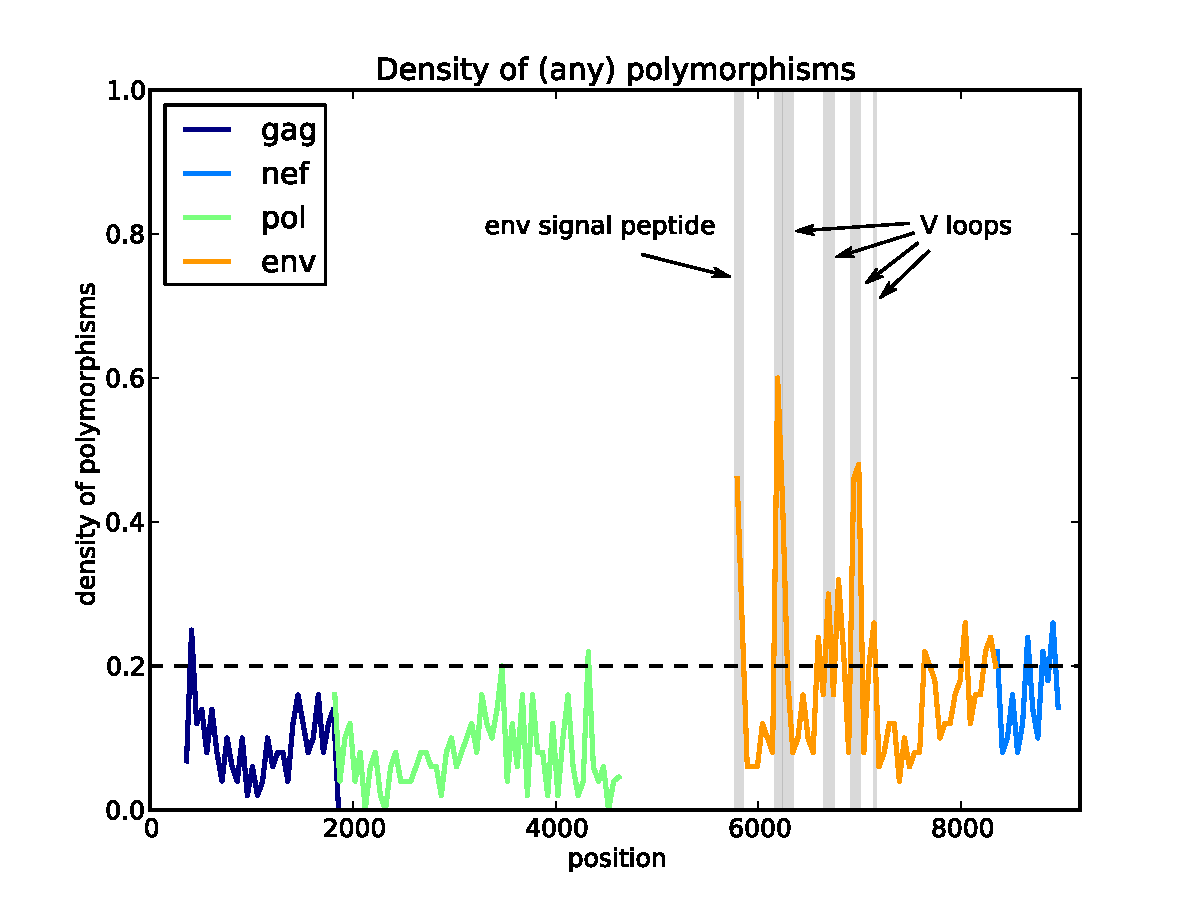
\includegraphics[width=0.49\linewidth]{Henn_density_polymorphisms}}
\subfloat{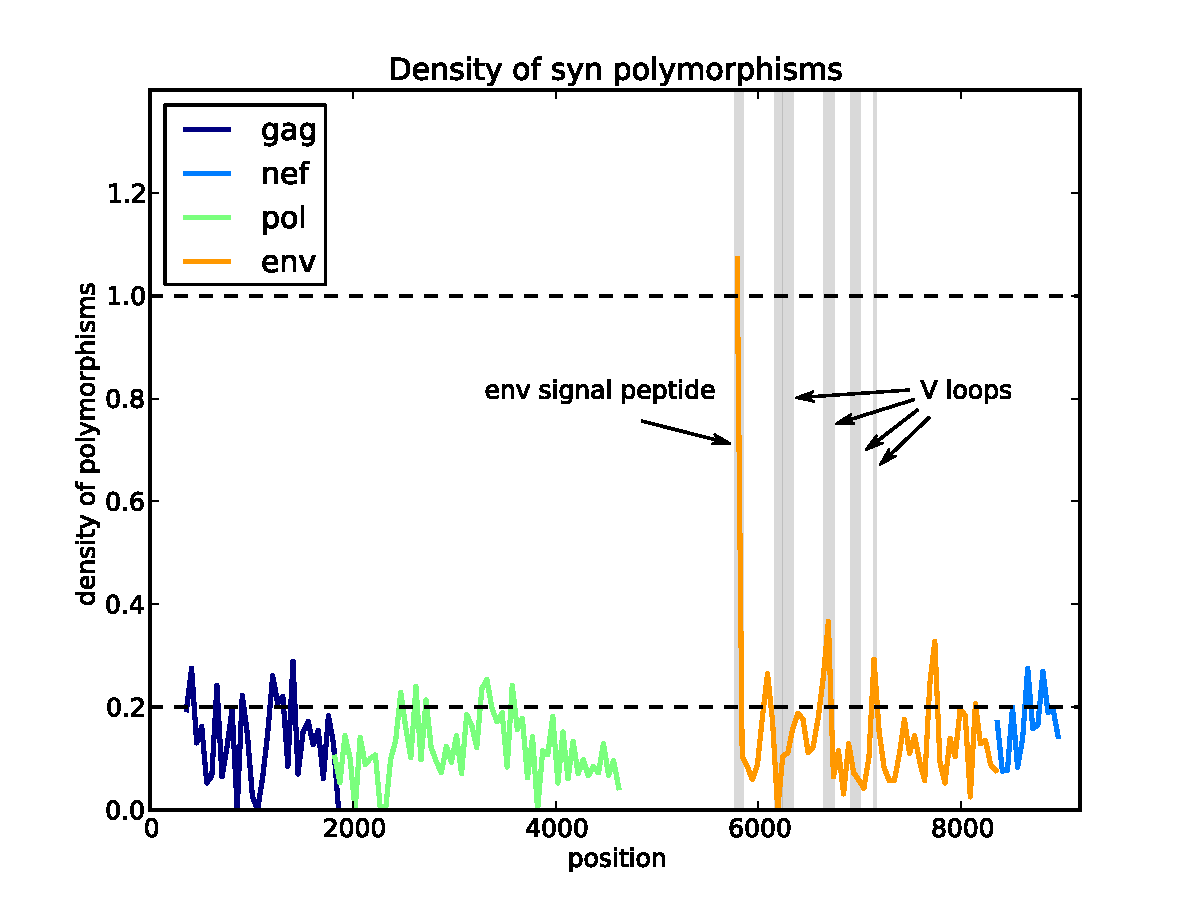
\includegraphics[width=0.49\linewidth]{Henn_density_polymorphisms_syn_over_chances}}
\caption{The total density of polymorphisms (mostly nonsynonymous ones) is
highest in the V regions (left panel). The density of synonymous mutations only,
however, is not enriched there (right panel). This could be due to a more
deleterious effect of synonymous mutations.}
\end{center}
\end{figure}


\begin{figure}
\begin{center}
\subfloat{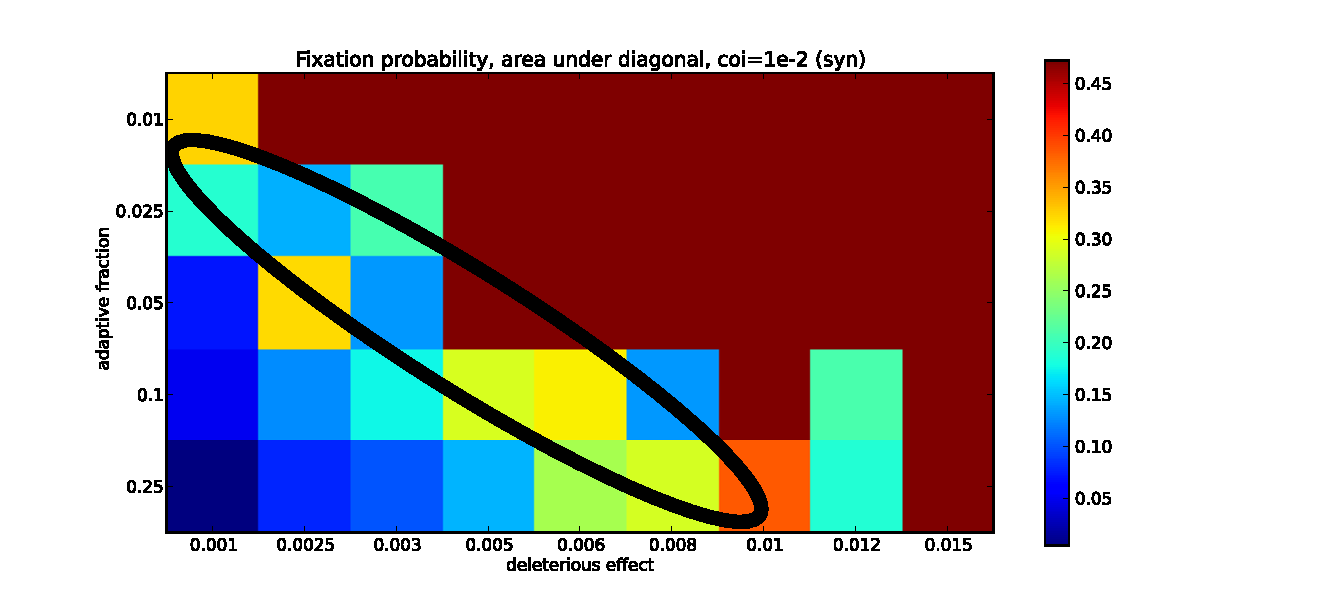
\includegraphics[width=0.49\linewidth]{fixation_loss_shortgenome_area_ada_frac_del_eff_coi_0_01_nescepi_6_heat.pdf}}
\subfloat{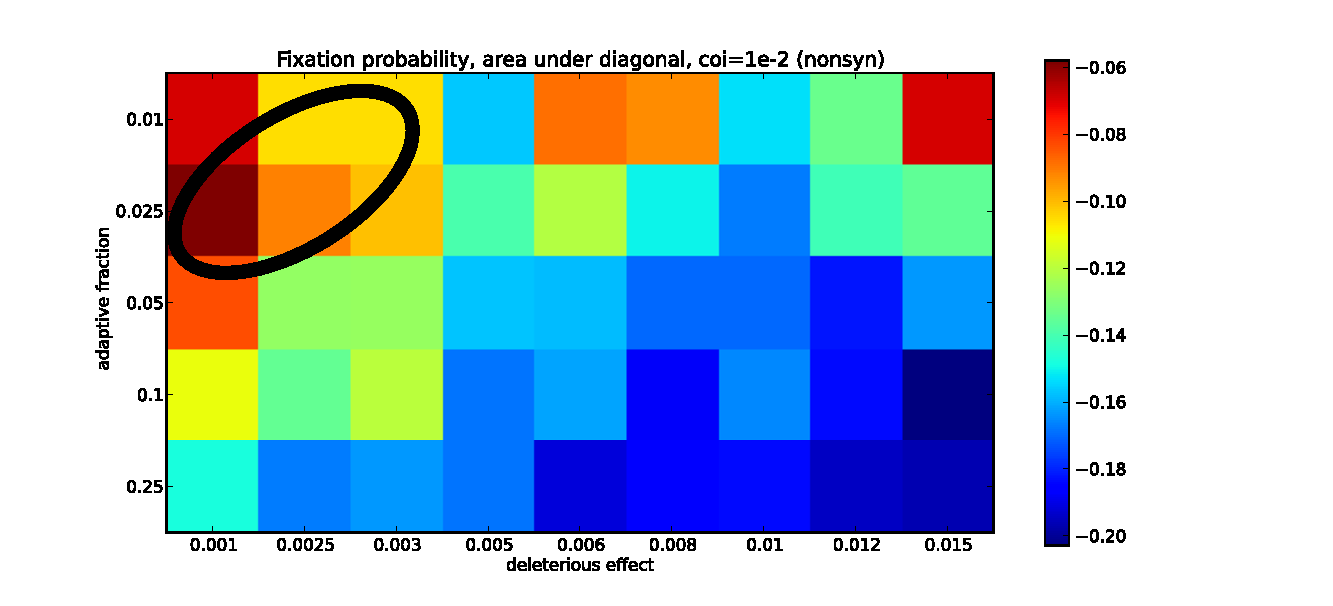
\includegraphics[width=0.49\linewidth]{fixation_loss_shortgenome_area_ada_frac_del_eff_coi_0_01_nescepi_6_nonsyn_heat.pdf}}

\caption{Simulations on the escape competition scenario show that the density of
 selective sweeps and the size of the deleterious effects of synonymous
 mutations are the main driving forces of the phenomenon. A convex fixation
 probability is recovered, as seen in the data, along the diagonal (left panel):
 more dense sweeps can support more deleterious linked mutations. The density of
 sweeps is limited, however, by the nonsynonymous fixation probability, which is
 quite close to neutrality (right panel). Moreover, strong competition between
 escape mutants is required, so that several escape mutants are ``found'' by HIV
within a few months of antibody production.}

\end{center}
\end{figure}

\section{Discussion}
\section{Methods}
\section*{Acknowledgements}

%%%%%%%%%%%%%%%%%%%%%%%%%%%%%%%%%%%%%%%%%%%%%%%%%%%%%%%%%%%%%%%%%%%%%%%%%
\bibliographystyle{natbib}
\bibliography{bib}
%%%%%%%%%%%%%%%%%%%%%%%%%%%%%%%%%%%%%%%%%%%%%%%%%%%%%%%%%%%%%%%%%%%%%%%%%
\end{document}
%%%%%%%%%%%%%%%%%%%%%%%%%%%%%%%%%%%%%%%%%%%%%%%%%%%%%%%%%%%%%%%%%%%%%%%%%

